\documentclass[a4paper]{article}

\usepackage[T1]{fontenc}
\usepackage[utf8]{inputenc}
\usepackage{polski}
\usepackage{graphicx}
\usepackage{hyperref}




\title{Programowanie Urządzeń Mobilnych \\ Laboratorium \\ \textbf{LISTA 1}}
\author{Rafał Lewandków}
\date{termin oddania: 04.11.2022}
\begin{document}
\maketitle
    

\section*{PhysicsQuiz - 10 pkt}

Wykonaj prostą aplikację będącą quizem fizycznym. Aplikacja posiada dwie aktywności. Pierwsza aktywność zawiera sam quiz. Druga aktywność pozwala poznać prawidłową odpowiedź na pytanie. Na wszystkie pytania można odpowiedzieć \textbf{TAK} lub \textbf{NIE}. Quiz posiada 10 pytań.

\begin{itemize}
\item \textbf{1 pkt} -- Zaprojektuj layout dla obu aktywności. Pierwsza aktywność posiada trzy przyciski oraz pole \textbf{TextView}

\begin{figure}[h]
\centering
\caption{Layout pierwszej aktywności}
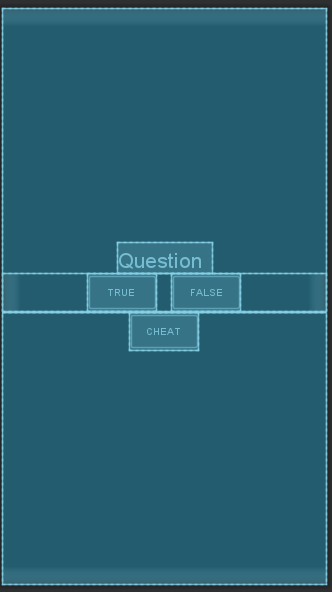
\includegraphics[scale=0.7]{l1.png}
\end{figure}

druga aktywność posiada tylko jedno pole \textbf{TextView}.

\item \textbf{1 pkt} -- Po naciśnięciu przycisku \textbf{TAK} lub \textbf{NIE} aplikacja przechodzi do następnego pytania

\item \textbf{1 pkt} -- Każda poprawna odpowiedź jest warta 10 pkt. Po zakończeniu quizu wyświetlane jest podsumowanie z ilością punktów, ilością poprawnych odpowiedzi, oraz liczbę oszustw.

\item \textbf{1 pkt} -- Po naciśnięciu przycisku \textbf{OSZUKUJ} przechodzimy do drugiej aktywności.

\item \textbf{3 pkt} -- Po ujawnieniu odpowiedzi w drugiej aktywności odejmowanych jest 15 pkt.

\item \textbf{2 pkt} -- Dodaj możliwość wyszukania treści pytania w internecie za pomocą mechanizmu \textbf{Implicit Intent}

\item \textbf{2 pkt} -- Zapewnij zachowanie danych za pomocą obiektu typu \textbf{Bundle}
\end{itemize}

\section*{OCENY}
Maxymalna liczba punktów: 10\\\
Oceny:\\
5.0 - 10 pkt\\
4.5 - 9 pkt\\
4,0 - 8 pkt\\
3,5 - 7 pkt\\
3,0 - 6 pkt
\end{document}

